
%% bare_jrnl_compsoc.tex
%% V1.4a
%% 2014/09/17
%% by Michael Shell
%% See:
%% http://www.michaelshell.org/
%% for current contact information.
%%
%% This is a skeleton file demonstrating the use of IEEEtran.cls
%% (requires IEEEtran.cls version 1.8a or later) with an IEEE
%% Computer Society journal paper.
%%
%% Support sites:
%% http://www.michaelshell.org/tex/ieeetran/
%% http://www.ctan.org/tex-archive/macros/latex/contrib/IEEEtran/
%% and
%% http://www.ieee.org/

%%*************************************************************************
%% Legal Notice:
%% This code is offered as-is without any warranty either expressed or
%% implied; without even the implied warranty of MERCHANTABILITY or
%% FITNESS FOR A PARTICULAR PURPOSE!
%% User assumes all risk.
%% In no event shall IEEE or any contributor to this code be liable for
%% any damages or losses, including, but not limited to, incidental,
%% consequential, or any other damages, resulting from the use or misuse
%% of any information contained here.
%%
%% All comments are the opinions of their respective authors and are not
%% necessarily endorsed by the IEEE.
%%
%% This work is distributed under the LaTeX Project Public License (LPPL)
%% ( http://www.latex-project.org/ ) version 1.3, and may be freely used,
%% distributed and modified. A copy of the LPPL, version 1.3, is included
%% in the base LaTeX documentation of all distributions of LaTeX released
%% 2003/12/01 or later.
%% Retain all contribution notices and credits.
%% ** Modified files should be clearly indicated as such, including  **
%% ** renaming them and changing author support contact information. **
%%
%% File list of work: IEEEtran.cls, IEEEtran_HOWTO.pdf, bare_adv.tex,
%%                    bare_conf.tex, bare_jrnl.tex, bare_conf_compsoc.tex,
%%                    bare_jrnl_compsoc.tex, bare_jrnl_transmag.tex
%%*************************************************************************


% *** Authors should verify (and, if needed, correct) their LaTeX system  ***
% *** with the testflow diagnostic prior to trusting their LaTeX platform ***
% *** with production work. IEEE's font choices and paper sizes can       ***
% *** trigger bugs that do not appear when using other class files.       ***                          ***
% The testflow support page is at:
% http://www.michaelshell.org/tex/testflow/


\documentclass[10pt,journal,compsoc]{IEEEtran}
%
% If IEEEtran.cls has not been installed into the LaTeX system files,
% manually specify the path to it like:
% \documentclass[10pt,journal,compsoc]{../sty/IEEEtran}
\usepackage{graphicx}
\usepackage[linesnumbered,ruled]{algorithm2e}
\usepackage{url}
\usepackage{epstopdf}
\usepackage{indentfirst}
\usepackage[tight,footnotesize]{subfigure}
\usepackage{amsmath}
\usepackage{amssymb}
\usepackage{multirow}

\newtheorem{Lemma}{Lemma}




% Some very useful LaTeX packages include:
% (uncomment the ones you want to load)


% *** MISC UTILITY PACKAGES ***
%
%\usepackage{ifpdf}
% Heiko Oberdiek's ifpdf.sty is very useful if you need conditional
% compilation based on whether the output is pdf or dvi.
% usage:
% \ifpdf
%   % pdf code
% \else
%   % dvi code
% \fi
% The latest version of ifpdf.sty can be obtained from:
% http://www.ctan.org/tex-archive/macros/latex/contrib/oberdiek/
% Also, note that IEEEtran.cls V1.7 and later provides a builtin
% \ifCLASSINFOpdf conditional that works the same way.
% When switching from latex to pdflatex and vice-versa, the compiler may
% have to be run twice to clear warning/error messages.






% *** CITATION PACKAGES ***
%
\ifCLASSOPTIONcompsoc
  % IEEE Computer Society needs nocompress option
  % requires cite.sty v4.0 or later (November 2003)
  \usepackage[nocompress]{cite}
\else
  % normal IEEE
  \usepackage{cite}
\fi
% cite.sty was written by Donald Arseneau
% V1.6 and later of IEEEtran pre-defines the format of the cite.sty package
% \cite{} output to follow that of IEEE. Loading the cite package will
% result in citation numbers being automatically sorted and properly
% "compressed/ranged". e.g., [1], [9], [2], [7], [5], [6] without using
% cite.sty will become [1], [2], [5]--[7], [9] using cite.sty. cite.sty's
% \cite will automatically add leading space, if needed. Use cite.sty's
% noadjust option (cite.sty V3.8 and later) if you want to turn this off
% such as if a citation ever needs to be enclosed in parenthesis.
% cite.sty is already installed on most LaTeX systems. Be sure and use
% version 5.0 (2009-03-20) and later if using hyperref.sty.
% The latest version can be obtained at:
% http://www.ctan.org/tex-archive/macros/latex/contrib/cite/
% The documentation is contained in the cite.sty file itself.
%
% Note that some packages require special options to format as the Computer
% Society requires. In particular, Computer Society  papers do not use
% compressed citation ranges as is done in typical IEEE papers
% (e.g., [1]-[4]). Instead, they list every citation separately in order
% (e.g., [1], [2], [3], [4]). To get the latter we need to load the cite
% package with the nocompress option which is supported by cite.sty v4.0
% and later. Note also the use of a CLASSOPTION conditional provided by
% IEEEtran.cls V1.7 and later.





% *** GRAPHICS RELATED PACKAGES ***
%
\ifCLASSINFOpdf
  % \usepackage[pdftex]{graphicx}
  % declare the path(s) where your graphic files are
  % \graphicspath{{../pdf/}{../jpeg/}}
  % and their extensions so you won't have to specify these with
  % every instance of \includegraphics
  % \DeclareGraphicsExtensions{.pdf,.jpeg,.png}
\else
  % or other class option (dvipsone, dvipdf, if not using dvips). graphicx
  % will default to the driver specified in the system graphics.cfg if no
  % driver is specified.
  % \usepackage[dvips]{graphicx}
  % declare the path(s) where your graphic files are
  % \graphicspath{{../eps/}}
  % and their extensions so you won't have to specify these with
  % every instance of \includegraphics
  % \DeclareGraphicsExtensions{.eps}
\fi
% graphicx was written by David Carlisle and Sebastian Rahtz. It is
% required if you want graphics, photos, etc. graphicx.sty is already
% installed on most LaTeX systems. The latest version and documentation
% can be obtained at:
% http://www.ctan.org/tex-archive/macros/latex/required/graphics/
% Another good source of documentation is "Using Imported Graphics in
% LaTeX2e" by Keith Reckdahl which can be found at:
% http://www.ctan.org/tex-archive/info/epslatex/
%
% latex, and pdflatex in dvi mode, support graphics in encapsulated
% postscript (.eps) format. pdflatex in pdf mode supports graphics
% in .pdf, .jpeg, .png and .mps (metapost) formats. Users should ensure
% that all non-photo figures use a vector format (.eps, .pdf, .mps) and
% not a bitmapped formats (.jpeg, .png). IEEE frowns on bitmapped formats
% which can result in "jaggedy"/blurry rendering of lines and letters as
% well as large increases in file sizes.
%
% You can find documentation about the pdfTeX application at:
% http://www.tug.org/applications/pdftex






% *** MATH PACKAGES ***
%
%\usepackage[cmex10]{amsmath}
% A popular package from the American Mathematical Society that provides
% many useful and powerful commands for dealing with mathematics. If using
% it, be sure to load this package with the cmex10 option to ensure that
% only type 1 fonts will utilized at all point sizes. Without this option,
% it is possible that some math symbols, particularly those within
% footnotes, will be rendered in bitmap form which will result in a
% document that can not be IEEE Xplore compliant!
%
% Also, note that the amsmath package sets \interdisplaylinepenalty to 10000
% thus preventing page breaks from occurring within multiline equations. Use:
%\interdisplaylinepenalty=2500
% after loading amsmath to restore such page breaks as IEEEtran.cls normally
% does. amsmath.sty is already installed on most LaTeX systems. The latest
% version and documentation can be obtained at:
% http://www.ctan.org/tex-archive/macros/latex/required/amslatex/math/





% *** SPECIALIZED LIST PACKAGES ***
%
%\usepackage{algorithmic}
% algorithmic.sty was written by Peter Williams and Rogerio Brito.
% This package provides an algorithmic environment fo describing algorithms.
% You can use the algorithmic environment in-text or within a figure
% environment to provide for a floating algorithm. Do NOT use the algorithm
% floating environment provided by algorithm.sty (by the same authors) or
% algorithm2e.sty (by Christophe Fiorio) as IEEE does not use dedicated
% algorithm float types and packages that provide these will not provide
% correct IEEE style captions. The latest version and documentation of
% algorithmic.sty can be obtained at:
% http://www.ctan.org/tex-archive/macros/latex/contrib/algorithms/
% There is also a support site at:
% http://algorithms.berlios.de/index.html
% Also of interest may be the (relatively newer and more customizable)
% algorithmicx.sty package by Szasz Janos:
% http://www.ctan.org/tex-archive/macros/latex/contrib/algorithmicx/




% *** ALIGNMENT PACKAGES ***
%
%\usepackage{array}
% Frank Mittelbach's and David Carlisle's array.sty patches and improves
% the standard LaTeX2e array and tabular environments to provide better
% appearance and additional user controls. As the default LaTeX2e table
% generation code is lacking to the point of almost being broken with
% respect to the quality of the end results, all users are strongly
% advised to use an enhanced (at the very least that provided by array.sty)
% set of table tools. array.sty is already installed on most systems. The
% latest version and documentation can be obtained at:
% http://www.ctan.org/tex-archive/macros/latex/required/tools/


% IEEEtran contains the IEEEeqnarray family of commands that can be used to
% generate multiline equations as well as matrices, tables, etc., of high
% quality.




% *** SUBFIGURE PACKAGES ***
%\ifCLASSOPTIONcompsoc
%  \usepackage[caption=false,font=footnotesize,labelfont=sf,textfont=sf]{subfig}
%\else
%  \usepackage[caption=false,font=footnotesize]{subfig}
%\fi
% subfig.sty, written by Steven Douglas Cochran, is the modern replacement
% for subfigure.sty, the latter of which is no longer maintained and is
% incompatible with some LaTeX packages including fixltx2e. However,
% subfig.sty requires and automatically loads Axel Sommerfeldt's caption.sty
% which will override IEEEtran.cls' handling of captions and this will result
% in non-IEEE style figure/table captions. To prevent this problem, be sure
% and invoke subfig.sty's "caption=false" package option (available since
% subfig.sty version 1.3, 2005/06/28) as this is will preserve IEEEtran.cls
% handling of captions.
% Note that the Computer Society format requires a sans serif font rather
% than the serif font used in traditional IEEE formatting and thus the need
% to invoke different subfig.sty package options depending on whether
% compsoc mode has been enabled.
%
% The latest version and documentation of subfig.sty can be obtained at:
% http://www.ctan.org/tex-archive/macros/latex/contrib/subfig/




% *** FLOAT PACKAGES ***
%
%\usepackage{fixltx2e}
% fixltx2e, the successor to the earlier fix2col.sty, was written by
% Frank Mittelbach and David Carlisle. This package corrects a few problems
% in the LaTeX2e kernel, the most notable of which is that in current
% LaTeX2e releases, the ordering of single and double column floats is not
% guaranteed to be preserved. Thus, an unpatched LaTeX2e can allow a
% single column figure to be placed prior to an earlier double column
% figure. The latest version and documentation can be found at:
% http://www.ctan.org/tex-archive/macros/latex/base/


%\usepackage{stfloats}
% stfloats.sty was written by Sigitas Tolusis. This package gives LaTeX2e
% the ability to do double column floats at the bottom of the page as well
% as the top. (e.g., "\begin{figure*}[!b]" is not normally possible in
% LaTeX2e). It also provides a command:
%\fnbelowfloat
% to enable the placement of footnotes below bottom floats (the standard
% LaTeX2e kernel puts them above bottom floats). This is an invasive package
% which rewrites many portions of the LaTeX2e float routines. It may not work
% with other packages that modify the LaTeX2e float routines. The latest
% version and documentation can be obtained at:
% http://www.ctan.org/tex-archive/macros/latex/contrib/sttools/
% Do not use the stfloats baselinefloat ability as IEEE does not allow
% \baselineskip to stretch. Authors submitting work to the IEEE should note
% that IEEE rarely uses double column equations and that authors should try
% to avoid such use. Do not be tempted to use the cuted.sty or midfloat.sty
% packages (also by Sigitas Tolusis) as IEEE does not format its papers in
% such ways.
% Do not attempt to use stfloats with fixltx2e as they are incompatible.
% Instead, use Morten Hogholm'a dblfloatfix which combines the features
% of both fixltx2e and stfloats:
%
% \usepackage{dblfloatfix}
% The latest version can be found at:
% http://www.ctan.org/tex-archive/macros/latex/contrib/dblfloatfix/




%\ifCLASSOPTIONcaptionsoff
%  \usepackage[nomarkers]{endfloat}
% \let\MYoriglatexcaption\caption
% \renewcommand{\caption}[2][\relax]{\MYoriglatexcaption[#2]{#2}}
%\fi
% endfloat.sty was written by James Darrell McCauley, Jeff Goldberg and
% Axel Sommerfeldt. This package may be useful when used in conjunction with
% IEEEtran.cls'  captionsoff option. Some IEEE journals/societies require that
% submissions have lists of figures/tables at the end of the paper and that
% figures/tables without any captions are placed on a page by themselves at
% the end of the document. If needed, the draftcls IEEEtran class option or
% \CLASSINPUTbaselinestretch interface can be used to increase the line
% spacing as well. Be sure and use the nomarkers option of endfloat to
% prevent endfloat from "marking" where the figures would have been placed
% in the text. The two hack lines of code above are a slight modification of
% that suggested by in the endfloat docs (section 8.4.1) to ensure that
% the full captions always appear in the list of figures/tables - even if
% the user used the short optional argument of \caption[]{}.
% IEEE papers do not typically make use of \caption[]'s optional argument,
% so this should not be an issue. A similar trick can be used to disable
% captions of packages such as subfig.sty that lack options to turn off
% the subcaptions:
% For subfig.sty:
% \let\MYorigsubfloat\subfloat
% \renewcommand{\subfloat}[2][\relax]{\MYorigsubfloat[]{#2}}
% However, the above trick will not work if both optional arguments of
% the \subfloat command are used. Furthermore, there needs to be a
% description of each subfigure *somewhere* and endfloat does not add
% subfigure captions to its list of figures. Thus, the best approach is to
% avoid the use of subfigure captions (many IEEE journals avoid them anyway)
% and instead reference/explain all the subfigures within the main caption.
% The latest version of endfloat.sty and its documentation can obtained at:
% http://www.ctan.org/tex-archive/macros/latex/contrib/endfloat/
%
% The IEEEtran \ifCLASSOPTIONcaptionsoff conditional can also be used
% later in the document, say, to conditionally put the References on a
% page by themselves.




% *** PDF, URL AND HYPERLINK PACKAGES ***
%
%\usepackage{url}
% url.sty was written by Donald Arseneau. It provides better support for
% handling and breaking URLs. url.sty is already installed on most LaTeX
% systems. The latest version and documentation can be obtained at:
% http://www.ctan.org/tex-archive/macros/latex/contrib/url/
% Basically, \url{my_url_here}.





% *** Do not adjust lengths that control margins, column widths, etc. ***
% *** Do not use packages that alter fonts (such as pslatex).         ***
% There should be no need to do such things with IEEEtran.cls V1.6 and later.
% (Unless specifically asked to do so by the journal or conference you plan
% to submit to, of course. )


% correct bad hyphenation here
\hyphenation{op-tical net-works semi-conduc-tor}


\begin{document}
%
% paper title
% Titles are generally capitalized except for words such as a, an, and, as,
% at, but, by, for, in, nor, of, on, or, the, to and up, which are usually
% not capitalized unless they are the first or last word of the title.
% Linebreaks \\ can be used within to get better formatting as desired.
% Do not put math or special symbols in the title.
\title{Scalable $K$-Order LCP Array Construction for Massive Data}
%
%
% author names and IEEE memberships
% note positions of commas and nonbreaking spaces ( ~ ) LaTeX will not break
% a structure at a ~ so this keeps an author's name from being broken across
% two lines.
% use \thanks{} to gain access to the first footnote area
% a separate \thanks must be used for each paragraph as LaTeX2e's \thanks
% was not built to handle multiple paragraphs
%
%
%\IEEEcompsocitemizethanks is a special \thanks that produces the bulleted
% lists the Computer Society journals use for "first footnote" author
% affiliations. Use \IEEEcompsocthanksitem which works much like \item
% for each affiliation group. When not in compsoc mode,
% \IEEEcompsocitemizethanks becomes like \thanks and
% \IEEEcompsocthanksitem becomes a line break with idention. This
% facilitates dual compilation, although admittedly the differences in the
% desired content of \author between the different types of papers makes a
% one-size-fits-all approach a daunting prospect. For instance, compsoc
% journal papers have the author affiliations above the "Manuscript
% received ..." text while in non-compsoc journals this is reversed. Sigh.

\author{Yi~Wu,
        Wei~Jun~Liu,
        Ge~Nong,
        and Wai~Hong~Chan% <-this % stops a space
\IEEEcompsocitemizethanks{
\IEEEcompsocthanksitem Y.~Wu, J.~Liu, G.~Nong are with the Department of Computer Science and Technology, Sun Yat-sen University, Guangzhou, China.
\IEEEcompsocthanksitem G.~Nong is with SYSU-CMU Shunde International Joint Research Institute, Shunde, China.
E-mail: issng@mail.sysu.edu.cn
\IEEEcompsocthanksitem W.~Chan is with the Department of Mathematics and Information Technology, Hong Kong Institute of Education, Hong Kong.
}}

% note the % following the last \IEEEmembership and also \thanks -
% these prevent an unwanted space from occurring between the last author name
% and the end of the author line. i.e., if you had this:
%
% \author{....lastname \thanks{...} \thanks{...} }
% ^------------^------------^----Do not want these spaces!
%
% a space would be appended to the last name and could cause every name on that
% line to be shifted left slightly. This is one of those "LaTeX things". For
% instance, "\textbf{A} \textbf{B}" will typeset as "A B" not "AB". To get
% "AB" then you have to do: "\textbf{A}\textbf{B}"
% \thanks is no different in this regard, so shield the last } of each \thanks
% that ends a line with a % and do not let a space in before the next \thanks.
% Spaces after \IEEEmembership other than the last one are OK (and needed) as
% you are supposed to have spaces between the names. For what it is worth,
% this is a minor point as most people would not even notice if the said evil
% space somehow managed to creep in.



% The paper headers
%\markboth{Journal of \LaTeX\ Class Files,~Vol.~13, No.~9, September~2014}%
%{Shell \MakeLowercase{\textit{et al.}}: Bare Demo of IEEEtran.cls for Computer Society Journals}
% The only time the second header will appear is for the odd numbered pages
% after the title page when using the twoside option.
%
% *** Note that you probably will NOT want to include the author's ***
% *** name in the headers of peer review papers. ***
% You can use \ifCLASSOPTIONpeerreview for conditional compilation here if
% you desire.



% The publisher's ID mark at the bottom of the page is less important with
% Computer Society journal papers as those publications place the marks
% outside of the main text columns and, therefore, unlike regular IEEE
% journals, the available text space is not reduced by their presence.
% If you want to put a publisher's ID mark on the page you can do it like
% this:
%\IEEEpubid{0000--0000/00\$00.00~\copyright~2014 IEEE}
% or like this to get the Computer Society new two part style.
%\IEEEpubid{\makebox[\columnwidth]{\hfill 0000--0000/00/\$00.00~\copyright~2014 IEEE}%
%\hspace{\columnsep}\makebox[\columnwidth]{Published by the IEEE Computer Society\hfill}}
% Remember, if you use this you must call \IEEEpubidadjcol in the second
% column for its text to clear the IEEEpubid mark (Computer Society jorunal
% papers don't need this extra clearance.)



% use for special paper notices
%\IEEEspecialpapernotice{(Invited Paper)}



% for Computer Society papers, we must declare the abstract and index terms
% PRIOR to the title within the \IEEEtitleabstractindextext IEEEtran
% command as these need to go into the title area created by \maketitle.
% As a general rule, do not put math, special symbols or citations
% in the abstract or keywords.
\IEEEtitleabstractindextext{%
\begin{abstract}
    In this paper, a new method is presented to generate the $K$-order longest common prefix~(LCP) array for a size-$n$ input text $T$ with its suffix array, where the maximum LCP of a pair of suffixes of $T$ is truncated to be at most $K$ characters. We adapt LCP-BQT, a technique previously proposed for LCP computation of any b pairs of strings, to produce the LCP-array of $T$. A finger-printing function is also employed whereby the involved string comparisons are translated into integer comparisons that can be accomplished in constant time. This method can be applied on the internal memory and easily extended to both external memory and distributed computation models. For each of these models, the total time and space complexities are $\mathcal{O}(n\log K)$ and $\mathcal{O}(n)$, respectively. In particular, the method is scalable for a distributed model of $d$ computing nodes, where the time and space complexities are evenly divided onto each node as $\mathcal{O}((n\log K)/d)$ and $\mathcal{O}(n/d)$, respectively.
\end{abstract}

% Note that keywords are not normally used for peerreview papers.
\begin{IEEEkeywords}
$K$-order LCP array,suffix array, finger-printing, external and distributed models.
\end{IEEEkeywords}}


% make the title area
\maketitle


% To allow for easy dual compilation without having to reenter the
% abstract/keywords data, the \IEEEtitleabstractindextext text will
% not be used in maketitle, but will appear (i.e., to be "transported")
% here as \IEEEdisplaynontitleabstractindextext when the compsoc
% or transmag modes are not selected <OR> if conference mode is selected
% - because all conference papers position the abstract like regular
% papers do.
\IEEEdisplaynontitleabstractindextext
% \IEEEdisplaynontitleabstractindextext has no effect when using
% compsoc or transmag under a non-conference mode.



% For peer review papers, you can put extra information on the cover
% page as needed:
% \ifCLASSOPTIONpeerreview
% \begin{center} \bfseries EDICS Category: 3-BBND \end{center}
% \fi
%
% For peerreview papers, this IEEEtran command inserts a page break and
% creates the second title. It will be ignored for other modes.
\IEEEpeerreviewmaketitle



\IEEEraisesectionheading{\section{Introduction}\label{sec:introduction}}
Suffix array~(SA)~\cite{Manber1993} is a succinct data structure for full-text indexing. In conjunction with the longest common prefix~(LCP) array, SA can emulate a bottom-up or top-down traversal of the corresponding suffix tree and thus becomes popular for a variety of string processing tasks previously tackled by suffix tree~\cite{Abouelhodaa2004}. The SA construction problem has been deeply investigated in the past decades~\cite{Puglisi2007}. Some of the prior works on internal model establish SA by means of the induced-copying technique, in which unordered suffixes are induced from the sorted ones~\cite{Burkhardt2003,Manzini2004,Sch��rmann2007}. These methods are fast in practice but their worst-case asymptotic complexity is super-linear. There exist several time-linear algorithms and the majority of them are based on the recursion technique previously proposed for suffix tree construction~\cite{Farach1997}. The idea behind the technique is analogous to that of induced-copying, but the sibling is conducted in a recursive way. Particularly, the sorting procedure is comprised of a recursion phase followed by a merging phase, where a subset of suffixes is selected and sorted recursively in advance and the sorting result is further employed to facilitate the processing of the remaining groups during the merging phase~\cite{Ko2003,Kim2004,K\"{a}rkk\"{a}inen2003}. However, these algorithms have large constant factors in both time and space complexity, leading to an actual performance far from being satisfactory. This situation changes with the emergence of SA-IS~\cite{nong2011}, where a refined implementation provided by Yuta~(https://sites.google.com/site/yuta256/sais/) demonstrates that the novel approach can outperform almost all the existing linear and non-linear algorithms in internal memory.

The LCP-array construction problem has attracted much attention since the introduction of the data structure~\cite{Manber1993}. Kasai et al. proposed the first linear time construction method, which builds the array very fast using T, SA and inverse SA~\cite{Kasai2001}. Manzini et al. adapted the method to reduce the space requirement at the cost of an expansion in running time~\cite{Manzini2004-2}. K?rkk?inen et al. described an algorithm to construct the Permuted LCP-array, which can be transformed to the classical LCP-array in linear time~\cite{K?rkk?inen2009}. Until now, the most time and space efficient SA and LCP-array construction algorithms designed for random access memory~(RAM) model are based on the induced sorting principle~\cite{Fischer11}. However, the methods suffer from a great performance degradation due to the problem of pool locality accesses when extended from internal memory to external memory and distributed models.

However, great improvements in data sampling techniques have created new challenges as the ever-increasing data sets can no longer be processed internally. To close the gap, recently, three novel algorithms~\cite{Nong15, Bingmann12, Nong14} have been designed to adapt the internal SA construction algorithm SA-IS~\cite{nong2011} for sorting suffixes in external memory and achieved remarkable performance gains against the previous state-of-the-art~\cite{Dementiev08}. In particular, the eSAIS algorithm~\cite{Bingmann12} can also produce the LCPA together with the construction of suffix array, where the overhead of time and I/O volume is twice as that of the plain SA construction. The eGSA algorithm~\cite{Felipe2013} enables the simultaneous computation of SA and LCPA for data sets composed of multiple strings of variable-lengths by using multi-way merge-sort, where the time spent in construction is reduced to one-third of eSAIS. The exLCP algorithm~\cite{Markus2012} is a lightweight LCPA construction algorithm for very large collections of sequences, where the Burrow-Wheeler transform is calculated at the same time to facilitate the computation. Given the suffix array as input, the LCPscan algorithm \cite{Juha2014} builds the LCPA from the permuted LCPA and inverse SA computed in advance. Compared with eSAIS, LCPscan requires less disk space and performs better in terms of the running time and I/O efficiency. While these algorithms achieve remarkable time and space performance, however, their designs are quite sophisticated and not trivial to be extended for parallel and distributed models so as to scale the performance by a cluster of computers, for example.

It has been observed from~\cite{Felipe2013} that the average LCPs are typically small for realistic data, especially in genome data sets such as protein and DNA. This motivated us to design a practical algorithm for computing the $K$-order LCPA of input string $T$, where the maximum LCP of any two suffixes in $T$ is assumed to be no more than $K<<|T|$~(e.g. $K=8192$).

The contributions of this work are mainly two aspects:
\begin{enumerate}
\item Our first contribution is to design and implement a $K$-order LCPA construction method applicable to typical internal and external memory models, which can build the LCPA in $\mathcal{O}(n\log K)$ time and $\mathcal{O}(n)$ space using the LCP batch querying technique~(LCP-BQT)~\cite{Philip2013} previously proposed for sparse SA construction. This method can be easily applied on both the internal and the external models. The program that we developed for the external memory model is composed of less than 600 code lines in C++.
\item The existing parallel construction algorithms are mainly designed for shared memory models such as bulk synchronous parallel and parallel random access machine~\cite{Shun2014,Deo2013}. Our second contribution is to parallelize the method in a distributed system consisting of $d$ computing nodes.
\end{enumerate}

The rest of the paper is organized as below.
Section~\ref{sec:construction_in_ram} introduces LCP-BQT and describes the algorithmic framework of the proposed method in the RAM model.
Section~\ref{sec:construction_in_em} and~\ref{sec:construction_in_distributed} extend the method to the external memory and distributed models, respectively.
Finally, we give the performance evaluation in Section~\ref{sec:experimental_results} and the conclusion in Section~\ref{sec:conclusion}.

\section{$K$-Order LCPA Construction in RAM}\label{sec:construction_in_ram}

\subsection{Notation}\label{subsec:basic_notations}

Consider an input text $T[0,n-1] =T[0]T[1]...T[n-1]$ of $n$ characters from an ordered alphabet $\Sigma$. We assume $T[n-1]$ to be a unique character alphabetically smaller than any characters in $T[0,n-2]$ and introduce the following notations for description clarity.

\begin{itemize}
\item ${\sf pre}(T,i)$ and ${\sf suf}(T,i)$: We write ${\sf pre}(T,i)$ to be the prefix of $T$ running from $T[0]$ to $T[i]$ and write ${\sf suf}(T,i)$ to be the suffix of $T$ running from $T[i]$ to $T[n-1]$.
\item $SA_T$: The suffix array of $T$, denoted by $SA_T$, is a permutation of integers $[0,n)$ such that ${\sf suf}(T,SA_T[0])<{\sf suf}(T,SA_T[1])<...<{\sf suf}(T,SA_T[n-1])$ in their lexicographic order.
\item ${\sf lcp}(i,j)$ and $LCPA_T$: We write ${\sf lcp}(i,j)$ to be the LCP length of ${\sf suf}(T,i)$ and ${\sf suf}(T,j)$. The LCPA of $T$, denoted by $LCPA_T$, consists of $n$ integers taken from $[0,n)$, where $LCPA_T[i]= {\sf lcp}(SA_T[i],SA_T[i-1])$.
\item $\Delta_{k}$: We denote $2^{\log n - k - 1}$ by $\Delta_{k}$.
\end{itemize}

\subsection{LCP Batch Querying Technique}\label{subsec:lcp_batch_querying_technique}

Given $T$ and a set of $b$ pairs of indices $P$, LCP-BQT computes ${\sf lcp}(i,j)$ for all pairs $(i,j)\in P$ in $\mathcal{O}(n\log b)$ time using $\mathcal{O}(n)$ RAM space. The main idea behind the technique is to find the indices $(i_{fin}, j_{fin})$ for $(i,j)$ such that $T[i,i_{fin}-1]=T[j,j_{fin}-1]$ and $T[i_{fin}] \neq T[j_{fin}]$. To do this, it initially assigns $P$ to $P_0$ and performs a loop of $\log b$ rounds on the set, where the goal of round $k\in [0,\log b)$ is to decide whether ${\sf lcp}(i_k,j_k) \le \Delta_k$ or not for each pair $(i_k,j_k)\in P_k$ and generate $P_{k+1}$ as the input for round $k+1$ as following: if $T[i_k,i_k+\Delta_k-1] \neq T[j_k,j_k+\Delta_k-1]$, then insert $(i_k,j_k)$ into $P_{k+1}$; otherwise, insert $(i_k+\Delta_k,j_k+\Delta_k)$ into $P_{k+1}$. The string comparison in concern can be carried out by scanning the two strings from left to right and literally comparing the characters in their lexicographic order. However, this operation takes $O(2^{\log n})$ time at worst and thus becomes a performance bottleneck.

As a solution to relieving the time overhead, the finger-printing function presented in~\cite{Karp1987} is introduced herein for transforming string comparisons to their integer counterparts that can be done in constant time. The finger-print~(FP) of $T[i,j]$, namely $FP[i,j]$, is calculated by the formula $FP[i,j] = \sum_{p=i}^{j} \delta^{j-p} \cdot T[p] \, mod \, L$, in which $L$ is a prime and $\delta$ is an integer randomly chosen from domain $[1,L)$. Obviously, two identical strings always have a common finger-print, while the converse is not true. Fortunately, it has been proved that the error probability of two different strings having a same finger-print can be ignored when $L$ is very large.

Following the above description, the 3-step algorithmic framework for round $k$ is given below.

\begin{enumerate}
\item Scan $T$ rightward to iteratively compute the finger-print of ${\sf pre}(0,l)$ by the formula $FP[0,l] = FP[0,l-1] \cdot \delta + T[l] \,\, mod \,\, L$ and store $FP[0,l]$ in the hash table if $l\in \{ \{i_k-1\}\cup\{j_k-1\}\cup\{i_k +\Delta_{k} - 1\}\cup\{j_k+ \Delta_{k} - 1\},(i_k,j_k)\in P_k\}$.
\item For each $l\in \{\{i_k\}\cup \{j_k\}$, $(i_k,j_k)\in P_k\}$, compute the finger-print of $T[l,l+\Delta_{k} - 1]$ by the formula $FP[l,l+ \Delta_{k} - 1]=FP[0,l+ \Delta_{k} - 1] - FP[0,l-1] \cdot \delta^{\Delta_{k}} \, mod \, L$, where $FP[0,l+ \Delta_{k} - 1]$ and $FP[0,l-1]$ can be retrieved from the hash table in amortized $\mathcal{O}(1)$ time.
\item For each pair $(i_k,j_k)\in P_k$, compare $FP[i_k,i_k+\Delta_{k} - 1]$ with $FP[j_k,j_k+\Delta_{k} - 1]$. If equal, insert $(i_k+\Delta_{k},j_k+\Delta_{k})$ into $P_{k+1}$; otherwise, insert $(i_k, j_k)$ into $P_{k+1}$.
\end{enumerate}

The following two properties remain invariant during the whole loop.

\begin{itemize}
\item At the beginning of round $k$, ${\sf lcp}(i_k,j_k) \le 2 \cdot \Delta_{k}$ for each pair $(i_k,j_k) \in P_k$.
\item At the end of round $k$, ${\sf lcp}(i_{k+1},j_{k+1}) \le \Delta_{k}$ for each pair $(i_{k+1},j_{k+1}) \in P_{k+1}$.
\end{itemize}

After the loop, we have ${\sf lcp}(i_{\log b},j_{\log b}) \le \frac{n}{b}$ for each pair $(i_{\log b},j_{\log b}) \in P_{\log b}$, and thus can compute ${\sf lcp}(i_{\log b}, j_{\log b})$ in $\mathcal{O}(\frac{n}{b})$ time by literally compare the characters in ${\sf suf}(T,i_{\log b})$ and ${\sf suf}(T,j_{\log b})$ from left to right. Let $i_{fin} = i_{\log b} + {\sf lcp}(i_{\log b}, j_{\log b})$ and $j_{fin}= j_{\log b} + {\sf lcp}(i_{\log b}, j_{\log b})$, then $i_{fin}$ and $j_{fin}$ are the position indices to the right side of $i$ and $j$ such that $T[i,i_{fin}-1] = T[j,j_{fin}-1]$ and $T[i_{fin}] \neq T[j_{fin}]$.

\begin{Lemma}
\label{thm:lcp:naive}
The LCP of any $b$ pairs of suffixes in $T$ can be correctly computed in $\mathcal{O}(n\log b)$ time using $\mathcal{O}(b)$ RAM space with a high probability.
\end{Lemma}
Proof. The time complexity of LCP-BQT is dominated by the loop of $\log b$ rounds, where each round takes $\mathcal{O}(n)$ time for step 1 to iteratively compute the finger-prints of ${\sf pre}(T,l)$, and $\mathcal{O}(b)$ time for steps 2-3 to compute and compare the finger-prints of strings. The space in need is limited to $\mathcal{O}(b)$ words by employing a hash table for storing and retrieving the finger-prints.


\subsection{Details}\label{subsec:implementation_in_ram}

We exploit the use of LCP-BQT by converting the K-order LCPA construction problem to the computation of ${\sf lcp}(i,j)$ for all pairs of position indices in $\{(SA_T[1], SA_T[0]),(SA_T[2], SA_T[1])\ldots (SA_T[n], SA_T[n-1])\}$. For presentation clarity, parameters and notations listed below are introduced to the design of internal memory algorithm lcpa-ram, where $i\in [0,n)$ and $k\in [0,\log K)$.

\begin{itemize}
\item $CP_k$ and $PP_k$: integer arrays of size $2n$, in which the two substrings $T[CP_k[2i],CP_k[2i+1]]$ and $T[PP_k[2i],PP_k[2i+1]]$ are compared to determine their LCP.
\item $ICP_k$ and $IPP_k$: integer arrays of size $2n$, which are produced by radix-sorting $CP_k$ and $PP_k$, respectively.
\item $HT$: a hash table for storing and retrieving finger-prints of ${\sf pre}(T,i)$, where $i\in \{CP_k[j] \cup PP_k[j], j\in[0,2n)\}$.
\end{itemize}




\begin{algorithm}[hbtp!]
\caption{Compute $K$-Order $LCPA_T$ in RAM}
\label{fig:alg:ram}
lcpa-ram($T$, $SA_T$, {\em n}, $K$, $HT$){\\
\SetAlgoNoLine
Scan $SA_T$ rightward to produce $CP_0$ and $PP_0$. \\
Let $k = 0$. \\
\While{$k < \log K$}{
\Indentp{-1em}
Radix-sort $CP_k$ and $PP_k$ to produce $ICP_k$ and $IPP_k$. \\
For $i\in [0,n)$, scan $T$ rightward to compute the finger-print of ${\sf pre}(T,i)$ and let $FP[0,i]=HT[i]$ if $i\in \{ICP_k[j] \cup IPP_k[j], j\in[0,2n)\}$. \\
For $i\in [0,n)$, scan $CP_k$ and $PP_k$ rightward to compute and compare $FP[CP_k[2i]+1,CP_k[2i+1]]$ and $FP[PP_k[2i]+1,PP_k[2i+1]]$ for generating $CP_{k+1}$ and $PP_{k+1}$. \\
Let $k = k +1$ and clear $HT$. \\
}
For $i\in [0,n)$, scan $T$, $CP_{\log K}$ and $PP_{\log K}$ rightward to compute $\Upsilon_i = {\sf lcp}(CP_{\log K}[2i],PP_{\log K}[2i])$. \\
For $i\in [0,n)$, let ${\sf lcp}(SA_T[i],SA_T[i-1])=CP_{\log K}[2i] +\Upsilon_i-SA_T[i]$. \\
}
\end{algorithm}



At the very beginning, Algorithm~\ref{fig:alg:ram} computes $CP_0$ and $PP_0$ as following: 1) $CP_0[2i]=SA_T[i]-1$ and $CP_0[2i+1]=SA_T[i]+ \Delta_0 - 1$; and 2) $PP_0[2i]=SA_T[i-1]-1$ and $PP_0[2i+1]=SA_T[i-1]+ \Delta_0 - 1$. When finishing the computation, it proceeds on to performing a loop of $\log K$ rounds in lines 4-9. A key operation in round $k$ is to radix-sorts entries in $CP_k$ and $PP_k$ for iteratively computing the finger-prints of ${\sf pre}(T,l)$. Afterward, these values are retrieved from the hash table to compute and compare the finger-prints of $T[CP_k[2i]+1,CP_k[2i+1]]$ and $T [PP_k[2i]+1,PP_k[2i+1]]$ for producing $CP_{k+1}$ and $PP_{k+1}$. More specifically, increase $CP_{k}[2i]$ and $PP_{k}[2i]$ by $\Delta_k$ and $CP_{k}[2i+1]$ and $PP_{k}[2i+1]$ by $\Delta_{k+1}$ if the two finger-prints are identical; otherwise, decrease $CP_{k}[2i+1]$ and $PP_{k}[2i+1]$ by $\Delta_{k+1}$. The algorithm then assigns $CP_k$ and $PP_k$ to $CP_{k+1}$ and $PP_{k+1}$, respectively. After the while-loop, it takes $\mathcal{O}(n)$ time to compute the LCP array in lines 10-11 as ${\sf lcp}(CP_{\log K}[2i],PP_{\log K}[2i]) \le 1$ holds for any $i \in [0,n)$. This leads us to the conclusion stated below.

\begin{Lemma}
\label{thm:lcp:ram}
Given $T$ and $SA_T$, the $K$-order $LCPA_T$ can be correctly computed in $\mathcal{O}(n\log K)$ time using $\mathcal{O}(n)$ RAM space with a high probability.
\end{Lemma}
Proof. With respect to time complexity, the while-loop spends $\mathcal{O}(n\log K)$ time computing $CP_{\log K}$ and $PP_{\log K}$. On the other respect, it demands $\mathcal{O}(n)$ internal space to maintain $HT$, $CP_k$ and $PP_k$.

\section{$K$-Order LCPA Construction in Disk}\label{sec:construction_in_em}

A hash table is employed in Algorithm~\ref{fig:alg:ram} to store the finger-prints for quick lookups. This is feasible in the RAM model, but not practical when {\em n} becomes larger as the table can not be wholly afforded internally anymore. For the purpose, we reformulate lcpa-ram to design a disk-friendly external memory algorithm, called lcpa-disk, where the finger-prints in use are sequentially retrieved from the external memory.

\subsection{Notation}

Given the RAM capacity $M$ in our external memory model, $T$ and $SA_T$ are evenly partitioned into $d=n/m$ blocks, where each block is of size $m=O(M)$ and thus can be processed as a whole in RAM. We extend $CP_k$ and $PP_k$ previously exploited in lcpa-ram to define their counterparts $ECP_k$ and $EPP_k$. Both of them consist of $2n$ entries and each entry is a tuple of $\langle idx, pos, fp \rangle$ as described below.
\begin{itemize}
\item $idx$: the index of the entry in $ECP_k/EPP_k$, where $ECP[i].idx=EPP[i].idx=i$.
\item $pos$: the ending position index of ${\sf pre}(0,pos)$ in $T$.
\item $fp$: the finger-print of ${\sf pre}(0,pos)$.
\end{itemize}

For $i\in [0,n)$, the $fp$ values of $ECP_k[2i]$ and $ECP_k[2i+1]$ are employed to figure out $FP[ECP_k[2i].pos+1, ECP_k[2i+1].pos]$ by the formula $ECP_k[2i+1].fp - ECP_k[2i].fp \cdot \delta^{\Delta_k} \, mod \, L$, where $FP[EPP_k[2i].pos+1, EPP_k[2i+1].pos]$ can be obtained in a similar way.

\subsection{Details}
Differentiate from Algorithm~\ref{fig:alg:ram}, lcpa-disk performs two runs of external memory sort to arrange fixed-size entries by their integer keys of $\log n$ bits during each round. Specifically, entries in $ECP_k$ and $EPP_k$ are sorted by $pos$ to form $IECP_k$ and $IEPP_k$ in line 5, and sorted back by $idx$ to their original order in line 7. The first sort is for iteratively computing the finger-print of ${\sf pre}(0,pos)$. During the process, we record the computation result in the $fp$ field of each entry instead of a hash table. After the second sort, these values are used to produce $ECP_{k+1}$ and $EPP_{k+1}$ following the same way adopted in lcpa-ram. Given $M=\Omega(nW)^{0.5}$, where $W$ is the size of {I/O} buffers large enough to amortize the overhead of accesses to disks, each run can be done in $\mathcal{O}(n)$ time and space by adopting a multi-way external memory radix-sort of two passes, of which the first pass sorts the lowest $0.5\log n$ bits and the second pass sorts the highest $0.5\log n$ bits. Thus we can come to the following statement.

\begin{Lemma}
\label{thm:lcp:em}
Given $T$ and $SA_T$, the $K$-order $LCPA_T$ can be correctly computed in $O(n \log K)$ time using $O(n)$ disk space with a high probability.
\end{Lemma}

\begin{algorithm}[hbtp!]
\caption{Compute $K$-Order $LCPA_T$ in Disk}
\label{fig:alg:em}
lcpa-disk($T$, $SA_T$, {\em n}, $K$){\\
\SetAlgoNoLine
Scan $SA_T$ rightward to produce $ECP_0$ and $EPP_0$.\\
Let $k = 0$. \\
\While{$k < \log K$}{
\Indentp{-1em}
Radix-sort $ECP_k$ and $EPP_k$ by $pos$ to produce $IECP_k$ and $IEPP_k$. \\
For $i\in [0,n)$ and $j\in [0,2n)$, scan $T$ rightward to iteratively compute the finger-print of ${\sf pre}(T,i)$ and assign $FP[0,i]$ to $IECP_k[j].fp$ or $IEPP_k[j].fp$ if $IECP_k[j].pos = i$ or $IEPP_k[j].pos = i$. \\
Radix-sort $IECP_k$ and $IEPP_k$ by $idx$ to reproduce $ECP_k$ and $EPP_k$. \\
For $i \in [0,n)$, scan $ECP_k$ and $EPP_k$ rightward to compute and compare each pair of $(FP[ECP_k[2i].pos+1,ECP_k[2i+1].pos], FP[EPP_k[2i].pos+1,EPP_k[2i+1].pos])$ for generating $ECP_{k+1}$ and $EPP_{k+1}$. \\
Let $k = k + 1$. \\
}
For $i \in [0,n)$, scan $T$, $ECP_{\log K}$ and $EPP_{\log K}$ rightward to compute $\Upsilon_i = {\sf lcp}(ECP_{\log K}[2i].pos,EPP_{\log K}[2i].pos)$. \\
For $i \in [0,n)$, let ${\sf lcp}(SA_T[i],SA_T[i-1])=ECP_{\log K}[2i].pos+\Upsilon_i-SA_T[i]$.\\
}
\end{algorithm}

\subsection{Optimization}\label{subsec:optimization}

The $logK$-round while-loop is time-consuming in lcpa-disk. The algorithm can be adapted to generate $ECP_{k+2}\backslash EPP_{k+2}$ directly from $ECP_k\backslash EPP_k$ so that the number of loop rounds can be reduced by half. To this end, the procedure in lines 8-9 is reformulated as below.

\begin{enumerate}
\item Compute and compare the finger prints of $T[ECP_k[2i].pos+1,ECP_k[2i+1].pos]$ and $T[EPP_k[2i].pos+1,EPP_k[2i+1].pos]$. If equal, perform S2; otherwise, go to S3.
\item Compute and compare the finger-prints of $T[ECP_k[2i+1].pos+1,ECP_k[2i+1].pos+\Delta_{k+1}]$ and $T[EPP_k[2i+1].pos+1,EPP_k[2i+1].pos+\Delta_{k+1}]$. If equal, increase $ECP_k[2i].pos$ and $EPP_k[2i].pos$ by $\Delta_{k}+\Delta_{k+1}$ and $ECP_k[2i+1].pos$ and $EPP_k[2i+1].pos$ by $\Delta_{k+1}+\Delta_{k+2}$; otherwise, increase $ECP_k[2i].pos$ and $EPP_k[2i].pos$ by $\Delta_{k}$ and $ECP_k[2i+1].pos$ and $EPP_k[2i+1].pos$ by $\Delta_{k+2}$.
\item Compute and compare the finger-prints of $T[ECP_k[2i].pos+1,ECP_k[2i].pos+\Delta_{k+1}]$ and $T[EPP_k[2i].pos+1,EPP_k[2i].pos+\Delta_{k+1}]$. If equal, increase $ECP_k[2i].pos$ and $EPP_k[2i].pos$ by $\Delta_{k+1}$ and decrease $ECP_k[2i+1].pos$ and $EPP_k[2i+1].pos$ by $\Delta_{k+2}$; otherwise, decrease $ECP_k[2i+1].pos$ and $EPP_k[2i+1].pos$ by $\Delta_{k+1}+\Delta_{k+2}$.
\item Let $ECP_{k+2}=ECP_{k}$ and $EPP_{k+2}=EPP_{k}$.
\item Let $k = k+2$.
\end{enumerate}

This method, however, brings about a side effect that the workspace grows nearly twice as the prototype because each entry of $ECP/EPP$ is extended to hold two more finger-prints required for executing step 2 or 3. As with lcpa-disk, the finger-prints in use can be computed in $\mathcal{O}(1)$ time after the rightward scan of $T$ for computing and recording the finger-prints of corresponding prefix substrings. This method can be generalized to merge a number of successive loop rounds into one. We will show in Section~\ref{sec:experimental_results} that the revised algorithm, namely lcpa-disk-m, can achieve a substantial improvement against lcpa-disk in terms of speed.

\section{$K$-Order LCPA Construction in Distributed System}\label{sec:construction_in_distributed}

In what follows, we demonstrate how to parallelize our external memory algorithms in a distributed system consisting of $d$ computing nodes $\{N_0, N_1, ...N_{d-1}\}$. All nodes are interconnected with each other by a gigabit-switch operating in the full duplex mode where the internal and external memory capacities of each node are $M$ and $E~(>> M)$, respectively.

\subsection{Notation}

For $i\in [0,d)$ and $j\in [0,e)$, we evenly partition $T$ and $SA_T$ into $d=n/e$ blocks of size $e=\mathcal{O}(E)$ and allocate them among the computing nodes in a manner of one block per node as below. Similarly, entries in $ECP_k/EPP_k$ and $IECP_k/IEPP_k$ are also divided and distributed to all the computing nodes. Recall that the external memory algorithms lcpa-disk and lcpa-disk-m compute $ECP_{\log K}$ and $EPP_{\log K}$ via two runs of radix-sort externally. To emulate the procedure in our distributed system illustrated in Fig.\ref{fig:distributed_system}, we set up a group of sending/receiding buffers in each computing nodes for data transmission during the sorts. The following parameters and notations are introduced for description convenience, where $i,j\in [0,d)$ and $k\in [0,logK)$.

\begin{itemize}
\item $T_i$: the $i$-th block of $T$ on node $N_i$, where $T_i[j] = T[ie+j]$.
\item $SA_{T_i}$: the $i$-th block of $SA_T$ on node $N_i$, where $SA_{T_i}[j] = SA_T[ie+j]$.
\item $ECP_{i,k}/EPP_{i,k}$: the $i$-th block of $ECP_{i,k}/EPP_{i,k}$ on node $N_i$, where $ECP_{i,k}[j] = ECP_k[ie+j]$ and $EPP_{i,k}[j] = EPP_k[ie+j]$.
\item $IECP_{i,k}/IEPP_{i,k}$: the $i$-th block of $IECP_{i,k}/IEPP_{i,k}$ on node $N_i$, where $IECP_{i,k}[j] = IECP_k[ie+j]$ and $IEPP_{i,k}[j] = IEPP_k[ie+j]$.
\item $SB1_{i,j}$ and $SB2_{i,j}$: create two sending buffers $SB1_{i,j}$ and $SB2_{i,j}$ on node $i$ for every other node $j\ne i$, where $SB1_{i,j}$ and $SB2_{i,j}$ cache the entries of $ECP_{i,k}/IECP_{i,k}$ and $EPP_{i,k}/IEPP_{i,k}$ delivered to node $j$, respectively.
\item $RB1_{i,j}$ and $RB2_{i,j}$: create two receiving buffers $RB1_{i,j}$ and $RB2_{i,j}$ on node $i$ for every other node $j\ne i$, where $RB1_{i,j}$ and $RB2_{i,j}$ cache the entries of $ECP_{j,k}/IECP_{j,k}$ and $EPP_{j,k}/IEPP_{j,k}$ received from node $j$, respectively.
\end{itemize}

\begin{figure}[hbtp!]
  \centering
  \includegraphics[width=0.4\textwidth]{distributed_system.eps}
  \caption{Distributed System.}\label{fig:distributed_system}
\end{figure}


\subsection{Detail}

As with lcpa-disk, the distributed algorithm lcpa-ds performs two runs of radix-sorts to compute the $fp$ field of entries in $ECP_k$ and $EPP_k$ by using the sending and receiving buffers. In details, $N_i$ dispatches each entry $x$ in $ECP_{i,k}$ to the sending buffer $SB1_{i,j}$ satisfying $j = x.pos / e$ and delivers them to $N_j$. Upon the arrival of entries from other nodes, $N_j$ radix-sorts entries in $RB1$ by their $pos$ to form $IECP_{j,k}$. Then it scans $T$ from left to right to iteratively compute the finger-prints of required prefix substrings and record them in the $fp$ field of corresponding entries in $IECP_{j,k}$. After that, each entry $y$ in $IECP_{j,k}$ are cached in the sending buffer $SB1_{j,i}$ satisfying $i = y.pos /e$ and forwarded to $N_i$. $N_i$ radix-sorts the received entries in $RB1$ by their $idx$ to regenerate $ECP_{i,k}$. $N_i$ processes entries in $EPP_{i,k}$ following the same way with the help of $SB2_{i,j}$ and $RB2$. $ECP_{i,k+1}$ and $EPP_{i,k+1}$ can be computed by scanning $ECP_{i,k}$ and $EPP_{i,k}$ once. After the while-loop, the LCP array of $T[ie,ie+e)$ can be figured out in linear time according to $ECP_{i,{\log K}}$, $EPP_{i,{\log K}}$ and $SA_{T_i}$ residing on $N_i$. And we can simply concatenate the local LCP array on each node to form $LCP_T$.

\begin{algorithm}[hbtp!]
\caption{Compute $K$-Order $LCPA_T[ie,ie+e)$ on $N_i$}
\label{fig:alg:ds}
lcpa-ds($T_i$, $SA_{T_i}$, $e$, $K$){\\
\SetAlgoNoLine
Scan $T_i$ rightward to compute $ECP_{i,0}$ and $EPP_{i,0}$. \\
Let $k=0$. \\
For $j\in[0,d)$, create sending buffers $SB1_{i,j}$ and $SB2_{i,j}$. \\
Create receiving buffers $RB1_i$ and $RB2_i$. \\
\While{$k < \log K$}{
\Indentp{-1em}
Scan $SA_{T_i}$ rightward to compute $ECP_{i,k}$ and $EPP_{i,k}$. \\
For $j\in[0,d)$ and $p\in[0,2e)$, scan $ECP_{i,k}$ and $EPP_{i,k}$ rightward to cache $ECP_{i,k}[p]$ in $SB1_{i,j}$ or $EPP_{i,k}[p]$ in $SB2_{i,j}$ if $ECP_{i,k}[p].pos$ or $EPP_{i,k}[p].pos$ belongs to $[je,je+e)$. \\
For $j\in[0,d)$, send entries in $SB1_{i,j}$ and $SB2_{i,j}$ to $N_j$. \\
For $j\in[0,d)$, cache entries from $SB1_{i,j}$ and $SB2_{i,j}$ in $RB1_i$ and $RB2_i$. \\
Radix-sort entries in $RB1_i$ and $RB2_i$ by $pos$ to produce $IECP_{i,k}$ and $IEPP_{i,k}$. \\
For $p\in[0,e)$ and $q\in [0,2e)$, scan $T_i$ rightward to iteratively compute the finger-print of ${\sf pre}(T,ie+p)$ and assign $FP[0,ie+p]$ to $IECP_{i,k}[q].fp$ or $IEPP_{i,k}[q].fp$ if $IECP_{i,k}[q].pos = ie+p$ or $IEPP_{i,k}[q].pos = ie+p$. \\
For $j\in[0,d)$ and $p\in[0,2e)$, scan $IECP_i$ and $IEPP_i$ rightward to cache $IECP_{i,k}[p]$ in $SB1_{i,j}$ or $IEPP_{i,k}[p]$ in $SB2_{i,j}$ if $IECP_{i,k}[p].pos$ or $IEPP_{i,k}[p].pos$ belongs to $[je,je+e)$. \\
For $j\in[0,d)$, send entries in $SB1_{i,j}$ and $SB2_{i,j}$ to $N_j$. \\
For $j\in[0,d)$, cache entries from $SB1_{i,j}$ and $SB2_{i,j}$ in $RB1_i$ and $RB2_i$. \\
Radix-sort entries in $RB1_i$ and $RB2_i$ by $idx$ to reproduce $ECP_{i,k}$ and $EPP_{i,k}$. \\
For $p\in [0,e)$, scan $ECP_{i,k}$ and $EPP_{i,k}$ rightward to compute and compare the finger-prints of $T[ECP_{i,k}[2p].pos+1, ECP_{i,k}[2p+1].pos]$ and $T[EPP_{i,k}[2p].pos+1, EPP_{i,k}[2p+1].pos]$ for generating $ECP_{i,k+1}$ and $EPP_{i,k+1}$. \\
Let $k=k+1$. \\
}
For $p\in [0,e)$, scan $T_i$, $ECP_{i,\log K}$ and $EPP_{i,\log K}$ rightward to literally compute $\Upsilon_{i,p}={\sf lcp}(ECP_{i,\log K}[2p].pos,EPP_{i,\log K}[2p].pos)$. \\
For $p\in [0,e)$, let ${\sf lcp}(SA_{T_i}[p],SA_{T,i}[p-1])=ECP_{i,\log K}.pos + \Upsilon_{i,p} - SA_{T_i}[p]$. \\
}
\end{algorithm}

Note that, the internal memory is partitioned into two parts, where the first part is employed to maintain the sending/receiving buffers and the other part is used to establish I/O buffers for reading/writing entries of $ECP_{i,k}$ and $EPP_{i,k}$. High performance can be achieved if the memory capacity spared for these buffers is large enough to compensate the delay of data transmissions and amortize the overhead of I/O operations. Besides, the optimization adopted in lcpa-disk-m can also be used herein to accelerate the speed.

\begin{Lemma}
\label{thm:lcp:pdm}
Given $T$ and $SA_T$, the $K$-order $LCPA_T$ can be correctly computed in $\mathcal{O}(\frac{n}{d}\log K)$ time using $\mathcal{O}(\frac{n}{d})$ disk space on each computing node with a high probability.
\end{Lemma}
Proof. Algorithm~\ref{fig:alg:ds} performs radix-sorts among the computing nodes, where the overhead of time and space for data transmission sums up to $\mathcal{O}(e\log K)$ during the whole loop. This is because each node sends and receives $\mathcal{O}(e)$ entries per round.



\section{Experimental Results}\label{sec:experimental_results}

A series of experiments are conducted on a real data set collected from the web site \url{http://download.wikimedia.org/enwiki/} to evaluate the performance of {C++} programs for the external and distributed algorithms presented in Section~\ref{sec:construction_in_em} and~\ref{sec:construction_in_distributed}. The experimental platform for lcpa-disk and lcpa-disk-m is deployed on a computer equipped with 2 Intel Xeron E3-1220 CPUs, 4GiB RAM and a disk of 2TB capacity, while the one for lcpa-ds is set up in a distributed system consisting of four identical computers interconnected with a gigabit switch. Programs are compiled by gcc 4.8.4, running on Ubuntu 14.04 operating system.

Instead of to develop a radix sorter specific for our purpose, we use STXXL~\cite{Dementiev2007} to perform the external memory sorts in our programs. STXXL is a {C++} STL library designed for efficient computation in external memory, and freely available at \url{http://stxxl.sourceforge.net/}. Benefit from the powerful priority queues provided by STXXL, the codes for lcpa-disk, lcpa-disk-m and lcpa-ds are no more than 400, 600 and 700 lines, respectively.

Each result in the following tables and figures is a mean of two runs of the programs, where the running time and peak disk use are monitored by the shell command ``time" and ``stxxl::block\_manager", respectively.

\subsection{Performance Analysis for External Algorithms}

We show in Table.~\ref{tbl:disk_vs_diskm} the performance comparison of the external memory algorithms, where two time metrics $MT$ and $ST$ are employed for performance evaluation. Specifically, $ST$ is the running time in total and $MT$ is the time spent in processing each character per loop round. As can be seen, lcpa-disk-m merges every $W$ successive loop rounds into one for decreasing $ST$ at the cost of a growth in both $MT$ and the peak disk use $PD$. Particularly, given $K=8192$ and $W=2$, the program runs faster than that of lcpa-disk with varying corpora size $S$, where the number of loop rounds $RD$ for lcpa-disk and lcpa-disk-m are 13 and 7, respectively. However, when $W$ becomes larger, the cost of external memory sorts of each loop round for lcpa-disk-m increases more quickly than that for lcpa-disk, which leads to a performance degradation in terms of $ST$ under the same circumstances. In more details, for $W=2$ .... $W=3$ ....

\begin{table*}[htbp!]
\caption{$RD$, $MT$ in microseconds per (character $\cdot$ round), $ST$ in seconds and $PD$ in bytes per character, where $K=8192$, $N=2$ and $S$ varies from 200 MB to 2 GB.}
\label{tbl:disk_vs_diskm}
\centering
\begin{tabular}{|c|c|c|c|c|c|c|c|c|c|c|c|c|}
\hline
$S$ & \multicolumn{4}{c|}{lcpa-disk ($W=1$)} & \multicolumn{4}{c|}{lcpa-disk-m ($W = 2$)} & \multicolumn{4}{c|}{lcpa-disk-m ($W = 3$)}\\
\cline{2-13}
(MB) & $RD$ & $MT$ & $ST$ & $PD$ & $RD$ & $MT$ & $ST$ & $PD$ & $RD$ & $MT$ & $ST$ & $PD$\\
\hline
200 & 13 & 1.03 & 2803 & 30.94 & 7 & 1.33 & 1950 & 47.36 & 5 & 2.43 & 2541 & 77.52\\
\hline
400 & 13 & 1.11 & 6034 & 31.50 & 7 & 1.40 & 4108 & 47.36 & 5 & 2.20 & 4605 & 78.58\\
\hline
600 & 13 & 1.18 & 9650 & 31.58 & 7 & 1.48 & 6928 & 47.36 & 5 & 3.14 & 9860 & 130.86\\
\hline
800 & 13 & 1.34 & 14557 & 31.52 & 7 & 1.80 & 10547 & 47.38 & 5 & 3.06 & 12827 & 103.50\\
\hline
2048 & 13 & 1.72 & 48021 & 46.04 & 7 & 2.47 & 37029 & 60.48 & 5 & 4.59 & 49280 & 94.40\\
\hline
\end{tabular}
\centering
\end{table*}

As depicted in Fig.~\ref{fig:disk_vs_diskm}, the growth in $MT$ with an increasing $N$ indicates the non-linear scalability of the two algorithms, which is partly due to the priority queue of STXXL, where the container adopts a logarithmic-time sorter for sorting in external memory. This can be avoided by designing a specific radix-sorter with a sacrifice in the succinctness of the program.

\begin{figure}[hbtp!]
  \centering
  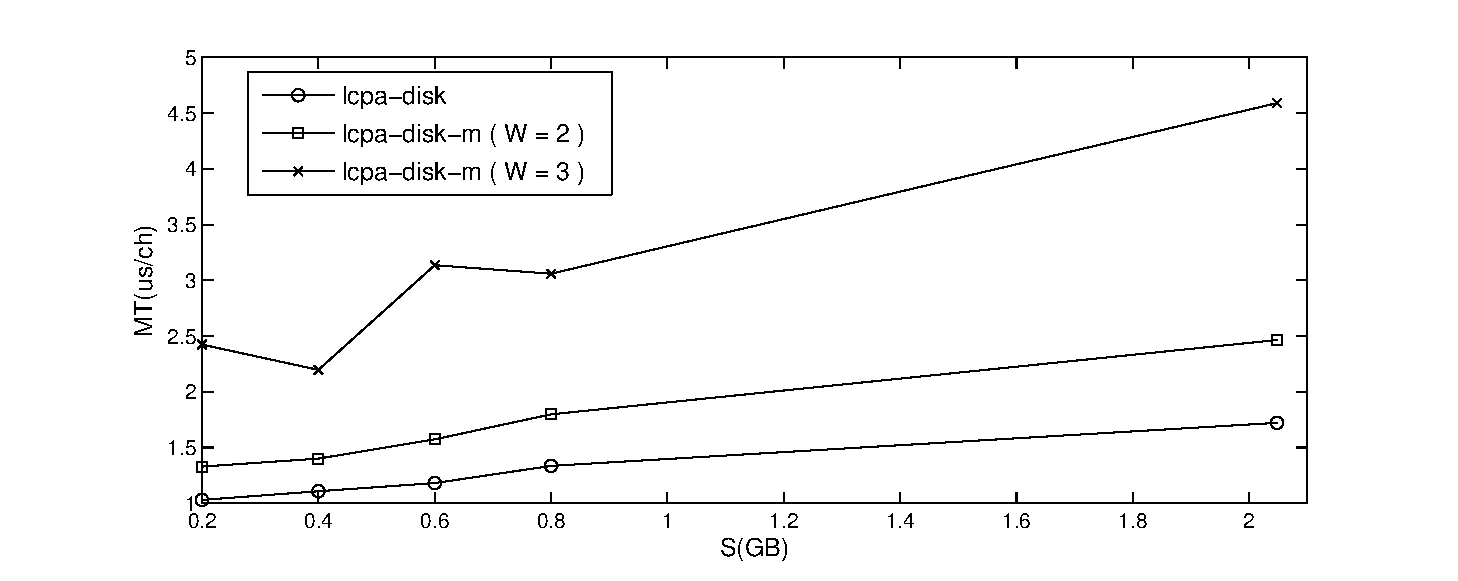
\includegraphics[width=0.5\textwidth]{disk_vs_diskm.eps}\\
  \caption{Performance comparison for lcpa-disk and lcpa-disk-m, where $K=8192$, $W=2$ and $S$ varies from 200 MB to 2 GB.}
  \label{fig:disk_vs_diskm}
\end{figure}

As reported in~\cite{Juha2014}, the disk space requirements for eSAIS and LCPscan are $65n$ and $21n$, respectively, while the peak disk use of the implementation for lcpa-disk-m~($W=2$) rises up to $61n$ for processing the 2 GB file. This indicates that {lcpa-disk-m} is more space demanding in comparison with the current best methods. However, we will show in the following paragraphs that the proposed method is easy to be implemented and strongly scalable for parallel and distributed models where the communication overhead on each node is balanced as $\mathcal{O}(\frac{n}{d})$.





\subsection{Performance Analysis for Distributed Algorithm}

It can be observed that lcpa-ds has a feature of strong scalability because the algorithm can be executed in parallel except for the external memory sorts. In Section~\ref{sec:construction_in_distributed}, we have shown how to emulate the sorter by using a group of sending/receiving buffers, where the communication overhead of the adapted algorithm on each computing node in~Fig.~\ref{fig:distributed_system} is upper-bounded by $\mathcal{O}(e)$. According to Amdahl's Law, the speed of lcpa-ds is probably $N-1$ times faster than that of lcpa-disk, where $N$ is the number of computing nodes in the distributed system. To validate the point, we provide lcpa-disk-m as a baseline to evaluate the performance of lcpa-ds.

As described in Table.~\ref{tbl:diskm_vs_ds}, lcpa-ds performs better than lcpa-disk-m in terms of $MT$ and $ST$ by a factor of 2, where $K=8192$, $W=2$ and $N=4$. Specifically, $MT$ for lcpa-ds increases from 0.71 to 1.24 when $S$ varies from 200 MB up to 2 GB. However, the performance gain obtained from parallelization is far less than we expected. One reason lies in the parallel overhead taken for data transmission among the computing nodes, but the dominate factor is the limited capacity of internal memory. To support the running of lcpa-ds, nearly half of the internal memory is allocated for maintaining the sending/receiving buffers on each computing node, leading to a substantial reduction in the internal memory $H$ available for I/O operations and external memory sorts. For further investigation, we show in Fig.~\ref{fig:stxxl_pq_impact} the performance variation of lcpa-disk with different $H$. It can be seen that a performance penalty occurs when $H$ decreases from 2.7 GB to 1.0 GB under the same conditions.

To evalute the scalability of lcpa-ds, we show in Fig.~\ref{xxx} the relation between $N$ and $MT$, where other parameters remain unchanged. It can be observed that xxx. The system's performance can be strengthen by establishing a specific global heap among the computing nodes instead of to use the delivering buffers.



\begin{table*}[htbp!]
\caption{$RD$, $MT$ in microseconds per (character $\cdot$ round), $ST$ in seconds and $PD$ in bytes per character, where $K=8192$, $W=2$, $N=4$ and $S$ varies from 200 MB to 2 GB.}
\label{tbl:diskm_vs_ds}
\centering
\begin{tabular}{|c|c|c|c|c|c|c|c|c|}
\hline
$S$ & $RD$ & \multicolumn{3}{c|}{lcpa-ds} & \multicolumn{3}{c|}{lcpa-disk-m} & Speedup\\
\cline{3-8}
(MB) & & $MT$ & $ST$ & $PD$ & $MT$ & $ST$ & $PD$ & (\%)\\
\hline
200 & 7 & 0.71 & 1038 & 0 & 1.33 & 1950 & 47.36 & 0.54 \\
\hline
400 & 7 & 0.72 & 2113 & 0 & 1.40 & 4108 & 47.36 & 0.52 \\
\hline
600 & 7 & 0.74 & 3235 & 0 & 1.48 & 6928 & 47.36 & 0.50 \\
\hline
800 & 7 & 0.78 & 4547 & 0 & 1.80 & 10547 & 47.38 & 0.43 \\
\hline
2048 & 7 & 1.24 & 18617 & 0 & 2.47 & 37029 & 60.48 & 0.50 \\
\hline
\end{tabular}
\centering
\end{table*}



\begin{figure}[hbtp!]
  \centering
  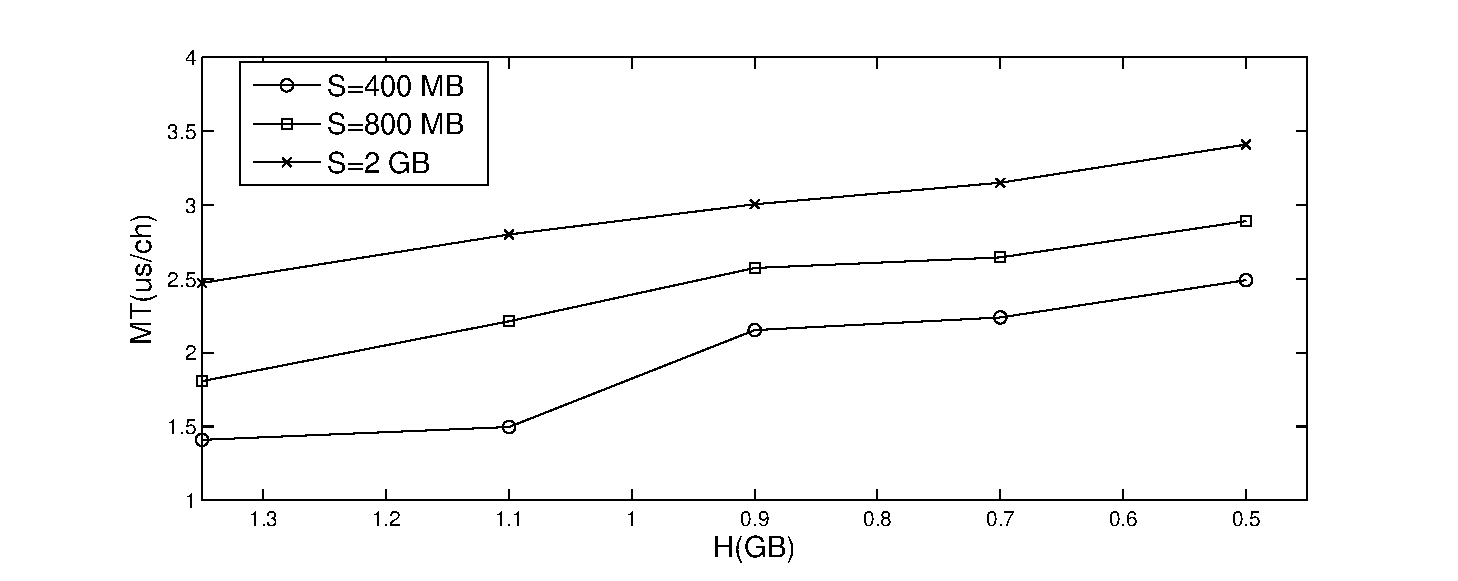
\includegraphics[width=0.5\textwidth]{stxxl_pq_impact.eps}\\
  \caption{Performance analysis for lcpa-disk-m with $H$ ranging in $\{2.7, 2.2, 1.8, 1.4, 1.0\}$ GB, where $K=8192$, $W=2$, $N=4$ and $S$ varies from 200 MB to 2 GB.}
  \label{fig:stxxl_pq_impact}
\end{figure}

\section{Conclusion}\label{sec:conclusion}

We present in this paper a practical $K$-order LCPA construction method that can be easily applied on both the internal memory and the external memory models. The program for lcpa-disk-m is less than 600 lines when using STXXL to implement the external sorts. We also show that the proposed method is straightforward to be extended for running on a typical distributed system of a cluster of $d$ computing nodes, where the time and space complexities are evenly divided onto each node as $\mathcal{O}(\frac{n}{d}\log K)$ and $\mathcal{O}(\frac{n}{d})$, respectively. The proposed algorithms are simple in design and universal for the RAM, disk and distributed models. Its implementations on all these models are not difficult and easily to be deployed.
A cluster of computers in a local area network are commonly available in practice, but there is currently lack of scalable LCPA construction algorithms for such a distributed model, in this sense, our algorithms provide a candidate solution to meet this demand. For further work, we now attempt to speed up the computation of finger-prints by GPU.

\bibliographystyle{unsrt}
\bibliography{bibfile}

\end{document}


